\documentclass[10pt,a4paper]{article}
\usepackage[utf8]{inputenc}
\usepackage[german]{babel}
\usepackage{mathrsfs}
\usepackage{amsmath}
\usepackage{amsfonts}
\usepackage{amssymb}
\usepackage{amsthm}
\usepackage[left=2cm,right=2cm,top=2cm,bottom=2cm]{geometry}
\usepackage{listings}
\usepackage{graphicx}

\begin{document}

\section{Aufgabe 7}

\subsection{Teil a}

\begin{align*}
  P(f) & = -8 \cdot \frac{(x - 2)(x - 3)(x - 6)}{(-2) \cdot (-3) \cdot (-6)} + 7 \cdot \frac{x(x - 2)(x - 6)}{(3 \cdot 1 \cdot (-3))} + 400 \cdot \frac{x(x - 2)(x - 3)}{6 \cdot 4 \cdot 3}\\
  & = 8 \cdot \frac{(x - 2)(x - 3)(x - 6)}{36} - 7 \cdot \frac{x(x - 2)(x - 6)}{9} + 400 \cdot \frac{x(x - 2)(x - 3)}{72}\\
\end{align*}

\subsection{Teil b}

\begin{equation}
  [x_{0}, x_{1}]f = \frac{8}{2} = 4
\end{equation}
\begin{equation}
  [x_{1}, x_{2}]f = \frac{7}{3 - 2} = 7
\end{equation}
\begin{equation}
  [x_{2}, x_{3}]f = \frac{400 - 7}{6 - 3} = \frac{393}{3} = 131
\end{equation}
\begin{equation}
  [x_{0}, x_{1}, x_{2}]f = \frac{7 - 4}{3} = 1
\end{equation}
\begin{equation}
  [x_{1}, x_{2}, x_{3}]f = \frac{131 - 7}{6 - 2} = \frac{124}{4} = 31
\end{equation}
\begin{equation}
  [x_{0}, x_{1}, x_{2}, x_{3}]f = \frac{31 - 1}{6} = 5
\end{equation}

\begin{equation}
  P(f) = -8 + x \cdot 4 + x(x - 2) + x(x - 2)(x - 3) \cdot 5
\end{equation}

\subsection{Teil c}

\begin{align*}
  P(f) & = -8 + x \cdot 4 + x(x - 2) + x(x - 2)(x - 3) \cdot 5\\
  & = -8 + 4x + x^{2} - 2x + 5(x^{2} - 2x)(x - 3)\\
  & = -8 + 2x + x^{2} + 5(x^{3} - 3x^{2} + 6x - 2x^{2})\\
  & = -8 + 2x + x^{2} + 5x^{3} - 15x^{2} + 30x - 10x^{2}\\
  & = 5x^{3} - 24x^{2} + 32x - 8
\end{align*}

\section{Aufgabe 8}

\begin{equation}
  T_{0}(x) = 1
\end{equation}
\begin{equation}
  T_{1}(x) = x
\end{equation}
\begin{equation}
  T_{2}(x) = 2x^{2} - 1
\end{equation}
\begin{equation}
  T_{3}(x) = 2x(2x^{2} - 1) - x
\end{equation}
\begin{equation}
  T_{4}(x) = 2x(2x(2x^{2} - 1) - x) - 2x^{2} + 1
\end{equation}
\begin{equation}
  T_{5}(x) = 2x(2x(2x(2x^{2} - 1) - x) - 2x^{2} + 1) - 2x(2x^{2} - 1) + x
\end{equation}
\begin{equation}
  T_{6}(x) = 2x(2x(2x(2x(2x^{2} - 1) - x) - 2x^{2} + 1) - 2x(2x^{2} - 1) + x) - 2x(2x(2x^{2} - 1) - x) + 2x^{2} + 1
\end{equation}
\begin{equation}
  T_{7}(x) = 2x(2x(2x(2x(2x(2x^{2} - 1) - x) - 2x^{2} + 1) - 2x(2x^{2} - 1) + x) - 2x(2x(2x^{2} - 1) - x) + 2x^{2} + 1) - 2x(2x(2x(2x^{2} - 1) - x) - 2x^{2} + 1) + 2x(2x^{2} - 1) - x
\end{equation}
\begin{equation}
  T_{8}(x) = 2x(2x(2x(2x(2x(2x(2x^{2} - 1) - x) - 2x^{2} + 1) - 2x(2x^{2} - 1) + x) - 2x(2x(2x^{2} - 1) - x) + 2x^{2} + 1) - 2x(2x(2x(2x^{2} - 1) - x) - 2x^{2} + 1) + 2x(2x^{2} - 1) - x) - 2x(2x(2x(2x(2x^{2} - 1) - x) - 2x^{2} + 1) - 2x(2x^{2} - 1) + x) + 2x(2x(2x^{2} - 1) - x) - 2x^{2} - 1
\end{equation}

\begin{lstlisting}
function y = tscheb (n, x)
  if n == 0
     y = ones(1, length(x));
  elseif n == 1
    y = x;
  else
    y = x .* 2 .* tscheb((n - 1), x) - tscheb((n - 2), x);
  endif
endfunction

hold on;

styles = ["y", "m", "c", "r", "g", "b", "y", "k", "m"];

x = -1:0.01:1;
for i = 0:8
  plot(x,
       tscheb(i, x),
       strcat(";T=", num2str(i), ";"),
       "Color", styles(i + 1),
       "LineWidth", 2);
endfor

hold off
\end{lstlisting}

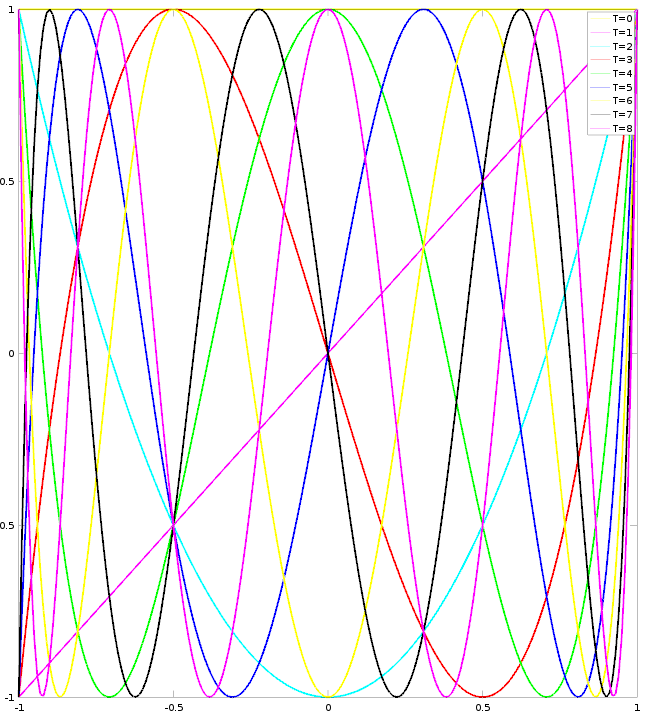
\includegraphics[width=250pt]{3_8.png}

\section{Aufgabe 9}

\subsection{Teil a}

\begin{equation}
  T_{n} \in \mathbb{P}_{n}
\end{equation}

\begin{proof}
  \begin{equation}
    T_{0} = \cos 0 = 1 \in P_{0}
  \end{equation}

  Sei $n > 0$ und die Behauptung für $n - 1$ bereits gezeigt.
  \begin{align*}
    T_{n} & = \cos(n \cdot \arccos x)\\
    & = \cos(\arccos x)\cos((n - 1)\arccos(x)) + \sin(\arccos x)\sin((n - 1)\arccos(x))\\^{}
  \end{align*}
\end{proof}

\subsection{Teil b}

\subsection{Teil c}

\section{Aufgabe 10}

\end{document}